We submitted a subset of our most promising lens candidates (112 targets) for the \emph{Hubble} SNAP program GO-15867 (PI: Huang),
\emph{Confirming Strong Galaxy Gravitational Lenses in the DESI Legacy Imaging Surveys}.
\ed{\hst not only provides higher angular resolution, but reaches fainter surface brightness due to the fainter background in space. 
This can reveal the presence of lensed galaxies with lower surface brightness, including those at higher redshifts that have been dimmed by $(1+z)^4$.
In addition, a NIR filter was chosen to make possible the detection of higher redshift sources that are beyond the optical ($grz$) reach of the DESI Legacy Surveys.
These two factors expand the depth
% , area, 
and redshift range of detectable arcs. 
Indeed, for a large number of systems in this program, the \hst NIR observations revealed additional lensed sources, often with a larger Einstein radius than the one seen in the respective discovery $grz$ images.}
The targets were chosen for two main science goals.
One, identifying the best systems for a future targeted search for lensed supernovae to measure the Hubble constant \citep[e.g.,][]{shu2018a, shu2021a}.
Lensed supernovae have been discovered in galaxy-scale \citep[e.g.,][]{goobar2023a, pierel2023a}, 
and cluster-scale lenses \citep[e.g.,][]{kelly2023a, frye2023a}.
Two, low-mass halo ($<10^9 M_\odot$) detection.
This is a powerful test of the cold dark matter (CDM) model, which predicts an abundance of low-mass halos, as subhalos or line-of-sight interlopers.
These do not host a galaxy and hence are invisible.
Beyond our local universe, they  are only detectable by their gravitational effect, especially in strong lensing systems \citep[e.g.,][]{vegetti2010a, cagan-sengul2022a}.
For this purpose, systems with a single galaxy as the main lens is usually preferred,
as these are considered to be easier to model and hence can yield low-mass halo detection with greater confidence.
\ed{However}, cluster-scale lenses have been used for this purpose too \citep[e.g.,][]{dai2020a}. 
To the degree possible, using the ground-based Legacy Surveys images, we chose half of our \hst targets to be galaxy-scale lenses and  
the other half, group/small cluster lenses.
Among strong lenses, being in-between galaxy-scale and cluster-scale, the latter category is somewhat understudied.
\ed{For example, in the SL2S program, 26 group-scale lenses were followed up with \hst observations \citep[][Table~3]{more2012a}.
Our program in the end observed a comparable number of group/small cluster lenses.}
This is likely due to the fact that these systems are outside of the previous selection windows: galaxy-scale lenses were discoverable in highly multiplexed fiber spectroscopy and cluster-scale lenses are more readily identified \ed{by eye in deep images}.
\ed{In contrast}, neural net based search methods applied to ground-based observations have discovered an abundance of strong lenses at the group to small cluster scales.
We would like to explore its potential for these two science goals.

All targets have $3 \times$399.23~sec exposure, 
for a total of 1197.7~sec, 
on WFC3 using the F140W filter in the NIR channel.
% There should be two exposures per visit, one visit per target, and identical specifications for all.
The targets were approximately centered in the WFC3 aperture, with no CR split, because we wanted to keep read noise down. 
Of the 112 systems submitted to \hst, 
a total of 53 were targeted. 
Two of them were not successfully observed due to the loss of the guide star.
% These exposures do not pack the orbit, but rather minimize the visit time within acceptable limits so as to achieve the best possible snapshot execution likelihood.
Of the 51 systems successfully observed, \hst confirmed all of them to be strong lenses, 
by revealing one or more arcs in each.\footnote{\ed{Of these}, DESI-118.8480+34.7610 is a known system \citep[][SDSS~J0755+3445]{shu2016b}, 
and it was observed in the optical by \hst WFC3 using UVIS F606W (GO-14189, PI: A. Bolton).}
The native pixel size is $0.13\twopr$, and each image is drizzled to $0.065''$.
In this \emph{Hubble} sample, 
\href{https://www.legacysurvey.org/viewer/?ra=025.4848&dec=+30.7585&layer=ls-dr9&pixscale=0.262&zoom=16}{DESI-025.4848+30.7585}\footnote{For the first mention of a system, we hyperlink the name to its Legacy Surveys DR9 image.}  has the faintest arcs.
It has a lens redshift of $z_d = 0.524$ from the extended Baryon Oscillation Spectroscopic Survey (eBOSS), 
which is further confirmed by DESI spectroscopy.
% $z_{d, phot} = 0.585\pm0.030$.
In the Legacy Surveys discovery image (see Figure~\ref{fig:hstpanel-1}), 
there appear to be a lensed arc (arc~1) to the SE of the elliptical galaxy at the center and a hint of a small arc (arc~2) to the NW of and just above the same elliptical galaxy.
Both are confirmed in the \hst image.
But \hst also reveals that just below arc~2, even closer to the lens, there appears to be a third arc (arc~3).
DESI provides the redshift for arc~1 ({$z_{s, 1} = 1.2223$, based on clear detection of the [\ion{O}{2}] doublet emission from DESI Year 1 data).
% ; Huang, Inchausti et al. in prep}).
% Much closer to the lens than this source, there appear to be two arc-like structure.
\citet{talbot2021a} analyzed the lens spectrum closely and found evidence for emission lines of a lensed source in the same eBOSS fiber, 
and determined its redshift at $z_{s, 2} = 1.216$.
The eBOSS fiber is $2''$ in diameter \citep{dawson2016a},
% \footnote{\url{https://www.sdss3.org/instruments/boss_spectrograph.php}}
and thus is capable of detecting emission features for an arc $\lesssim 1''$ away from the lens.
Therefore this redshift corresponds to either arc~3 ($0.87''$ from the lens) or arc~2 (at a distance of $1.20''$).
Arc~1 at 2.10$''$ is not likely.
% In this paper, we provide DESI redshifts for those systems for which these redshifts are needed for full confirmation as a strong lens.
In addition to this system, we will also provide spectroscopic redshifts from DESI and Keck for  DESI-165.4754-06.0423 (see Figure~\ref{fig:hstpanel-2}), 
for which we will show a lens model in \S\,\ref{sec:lens-model}.
DESI redshifts for other systems will be presented in Paper~II and future publications.

Figure~\ref{fig:hstpanel-1} shows the first eight systems in this sample.
These eight are representative of the type of lensing configuration for this \hst sample.
% In Figure~\ref{fig:desi165} 
% We have further confirmed a large fraction of them spectroscopically through the on-going DESI observations.
% The first batch of DESI strong lens spectroscopic results will be presented in Huang et al. (in prep).
% Among the targets in this program, the arcs were the faintest in the first system in Figure~\ref{fig:gal-lenses}, \href{https://www.legacysurvey.org/viewer?ra=25.4848&dec=30.7583&layer=ls-dr9&pixscale=0.262&zoom=16}{DESI-025.4848+30.7585}.
% \citet{talbot2021a} provided SDSS redshifts for the lens ($z_d = 0.524$) and one of the lensed sources ($z_{s, 1} = 1.216$).
% DESI confirms this source redshift and provides redshift for a second source ($z_{s, 2} = 1.2223$; Huang et al. in prep). 
% Among the galaxy-scale lenses (Figure~\ref{fig:gal-lenses}), 
We show the rest of the 51 systems in Figures~\ref{fig:hstpanel-2}~-~\ref{fig:hstpanel-6}. 
There are a number of striking systems.
In Figure~\ref{fig:hstpanel-1}, 
\ed{for \href{https://www.legacysurvey.org/viewer/?ra=4.2564&dec=-10.1530&layer=ls-dr9&pixscale=0.262&zoom=16}{DESI-004.2564-10.1530} and \href{https://www.legacysurvey.org/viewer/?ra=23.6765&dec=+4.5639&layer=ls-dr9&pixscale=0.262&zoom=16}{DESI-023.6765+04.5639}}, 
both group lenses, 
compared with the discovery images from the Legacy Surveys in the optical bands of $grz$,
the \hst NIR images reveal additional fainter arcs in each. 
This is true for a number of group-scale lensing systems in this sample.
\href{https://www.legacysurvey.org/viewer/?ra=72.0873&dec=-19.4174&layer=ls-dr9&pixscale=0.262&zoom=16}{DESI-072.0873-19.4172} (Figure~\ref{fig:hstpanel-2}) is an Einstein cross with a remarkable average lens-image separation of 3.95$\twopr$.
The photometric redshift for the lens is $z_{d, phot} = 0.967\pm0.167$.\footnote{Here and later in this paper, 
% unless otherwise noted, 
the photometric redshifts are from \citet{zhou2020a}.} 
% To the best of our knowledge, this is the second largest \ed{known} Einstein cross.
There appear to be at least three other elliptical galaxies with similar colors (and therefore similar redshifts) within or near the Einstein cross, 
though they are considerably smaller. 
Inspection of the environment around this system shows that the lensing galaxy is at the center of a high redshift cluster.
\ed{The presence of the Einstein cross, rarely seen for a group/cluster scale lens \citep[e.g.,][which shows an Einstein cross for a cluster lens with $z_d = 0.49$]{sheu2024a}, indicates that mass distribution is relaxed and highly symmetric within the Einstein radius, perhaps all the more unusual at such a high redshift. The modeling of this system is currently underway.}
% Another interesting system with a very large average image-lens separation, $\sim 9''$, is 
% \href{https://www.legacysurvey.org/viewer/?ra=278.8338&dec=46.1076&layer=ls-dr9&pixscale=0.262&zoom=16}{DESI-278.8338+46.1076} (Figure~\ref{fig:hstpanel-5}).
% The lens redshift is at $z_{d, phot} = 0.421\pm0.015$.
% From the forward modeling of source extraction pipeline \tractor \citep{lang2016a}, other nearby objects on the sky are morphologically typed as PSF.
% Thus these are either MW stars or distant quasars.
% Furthermore, they have very similar white-blue colors, and are almost certainly the same kind of objects.
% Some of these objects are DESI targets (yet to be observed), so their nature will be revealed soon.
% Thus the lensed arcs appear to be around a single galaxy. 
% But unlike the previous system, the lensing galaxy does appear to be at the center of a cluster.
% Besides the main arc (arc~1) with three (likely star forming) ``knots'', the Legacy Surveys image suggests there is another possible arc (arc~2),
% with a similar color,
% just below arc~1. 
% The \hst image certainly confirms arc~1 and appears to lend support to arc~2. 
% In addition, on the opposite side of the lens, 
% near the SW corner of the cutout image, 
% there appear to be a compact object with a slight elongation perpendicular to the line connecting it to the lens; this may be the counterarc to arc~1.
% Next to this compact object, there is a more diffuse object that appears to be an arclet --- this is  possibly the counterimages of and arc~2.
% The similarity in color between the main arcs and their putative counterimages supports this conjecture.
% {\color{red}Two near Einstein rings. Systems with sources at different redshifts.}
Other notable systems include: 
% Three systems 
a galaxy-scale lensing system that possibly has two multiply-imaged sources (\href{https://www.legacysurvey.org/viewer/?ra=133.3800&dec=+23.3653&layer=ls-dr9&pixscale=0.262&zoom=16}{DESI-133.3800+23.3652} in Figure~\ref{fig:hstpanel-2}, \ed{shown with arrows})
%\footnote{\href{https://www.legacysurvey.org/viewer/?ra=238.5690&dec=4.7276&layer=ls-dr9&pixscale=0.262&zoom=16}{DESI-238.5690+04.7276}  in Figure~\ref{fig:hstpanel-5} appears to possibly have two sources as well. Although preliminary lens modeling indicates these are two components of a single source.})
and two group-scale systems with multiple images of a background galaxy with complex structure 
(\href{https://www.legacysurvey.org/viewer/?ra=189.5370&dec=15.0309&layer=ls-dr9&pixscale=0.262&zoom=16}{DESI-189.5370+15.0309} in Figure~\ref{fig:hstpanel-3} with a doubly imaged background spiral galaxy, 
or two half ``cinnamon buns", and 
\href{https://www.legacysurvey.org/viewer/?ra=327.8408&dec=13.7884&layer=ls-dr9&pixscale=0.262&zoom=16}{DESI-327.8408+13.7884} in Figure~\ref{fig:hstpanel-6}, showing great details of a triply lensed spiral galaxy, \ed{which suggests a possible naked cusp configuration \citep[e.g.,][]{lewis2002a}}.
Finally, the \hst image of \href{https://www.legacysurvey.org/viewer/?ra=254.4235&dec=34.8161&layer=ls-dr9&pixscale=0.262&zoom=16}{DESI-254.4235+34.8162} (Figure~\ref{fig:hstpanel-5}) possibly reveals a radial counter arc very close to the lensing galaxy.

\clearpage
% , \ed{which can potentially be used to constrain the mass of the supermassive black hole at its center \citep[e.g.,][]{nightingale2023a}}.
% three images showing great details of the same spiral galaxy) 

% DESI-310.8019-06.1649 (three image with alternating parity).


%%% Don't delete:
%https://docs.google.com/presentation/d/1fTakr8mnK8Q4-73qR-K-D87auFSvxZ31Ap-fiBHL-OE/edit#slide=id.g124f7356344_0_69

%%% This is the AAS example figure
% \begin{figure}[ht!]
% \plotone{figs/gal-lenses-LS.pdf}
% \caption{The subscription (squares) and author publication (asterisks) 
% costs from 1991 to 2013. Subscription cost are on the left Y axis while
% the author costs are on the right Y axis. All numbers in US dollars and
% adjusted for inflation. The author charges also account for the change
% from page charges to digital quanta in April 2011.  \label{fig:general}}
% \end{figure}

\begin{minipage}{\linewidth}
\makebox[\linewidth]{  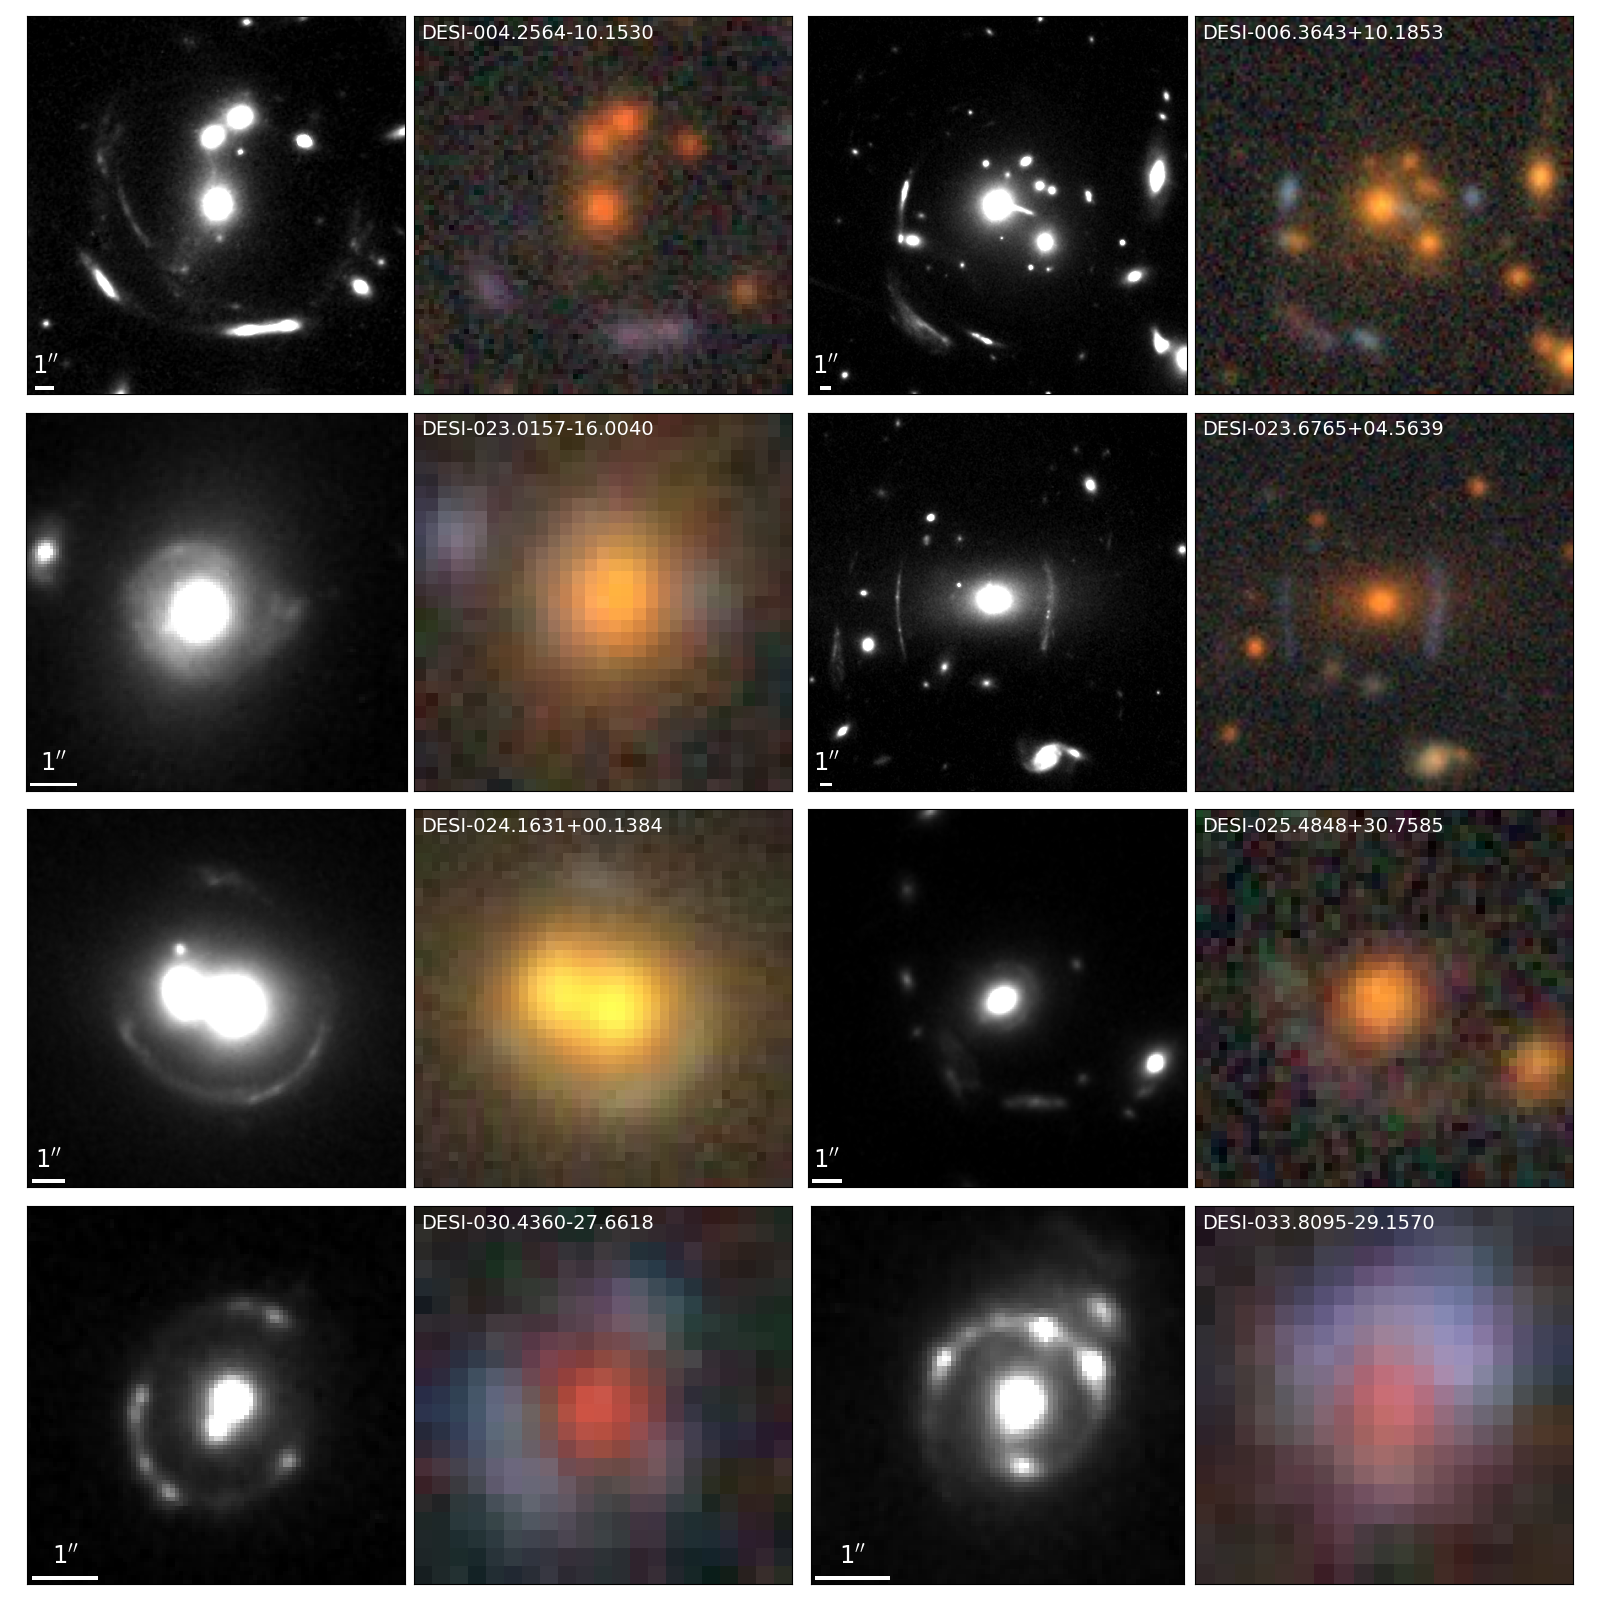
\includegraphics[keepaspectratio=true,scale=0.45]{figs/hst_panel1.png}}
\captionof{figure}{
The first eight of the 51 systems observed by the \hst SNAP program GO-15867. 
All were confirmed to be strong lenses by \hst with arc(s) in each clearly revealed.
For this and the next five figures (up to and including Figure~\ref{fig:hstpanel-6}): 
The naming convention is RA and Dec in decimal format.
% There are a number of striking systems (see text).
% One of the 26 systems with a single galaxy as the main lens ... The left panel shows the Legacy Surveys image for DESI-165.4754-06.0423 (discovery images).
North is up, and East to the left. 
The systems are arranged in ascending RA.
For each, we show the \hst WFC3 NIR F140W image (left)
% , drizzled to 0.065$\twopr$, 
and the Legacy Surveys optical image in $grz$ bands (right; these were the discovery images).
The eight systems in this panel are representative of the 51 systems in this \hst program: There are three group/small cluster scale lenses, DESI-004.2564-10.1530, DESI-006.3643+10.1853, and DESI-023.6765+04.5639.
For each of them, there are at least two sets of arcs. 
Compared with the Legacy Surveys optical image, 
the NIR \hst image revealed new arcs for the first and third system.
\ed{DESI-023.0157-16.0040, DESI-025.4848+30.7585, and DESI-033.8095-29.1570 are galaxy-scale lens} (for more on the lensing nature of DESI-025.4848+30.7585, see text).
Finally, DESI-024.16341+00.1384 and DESI-030.4360-27.6618 \ed{each have} two very close-by elliptical galaxies as the lens.}
% The first one at top left has the faintest arcs (see text).
% \S\ref{sec:lens-model} presents the lens model for this system.}
\label{fig:hstpanel-1}
\end{minipage}

\begin{minipage}{\linewidth}
\makebox[\linewidth]{  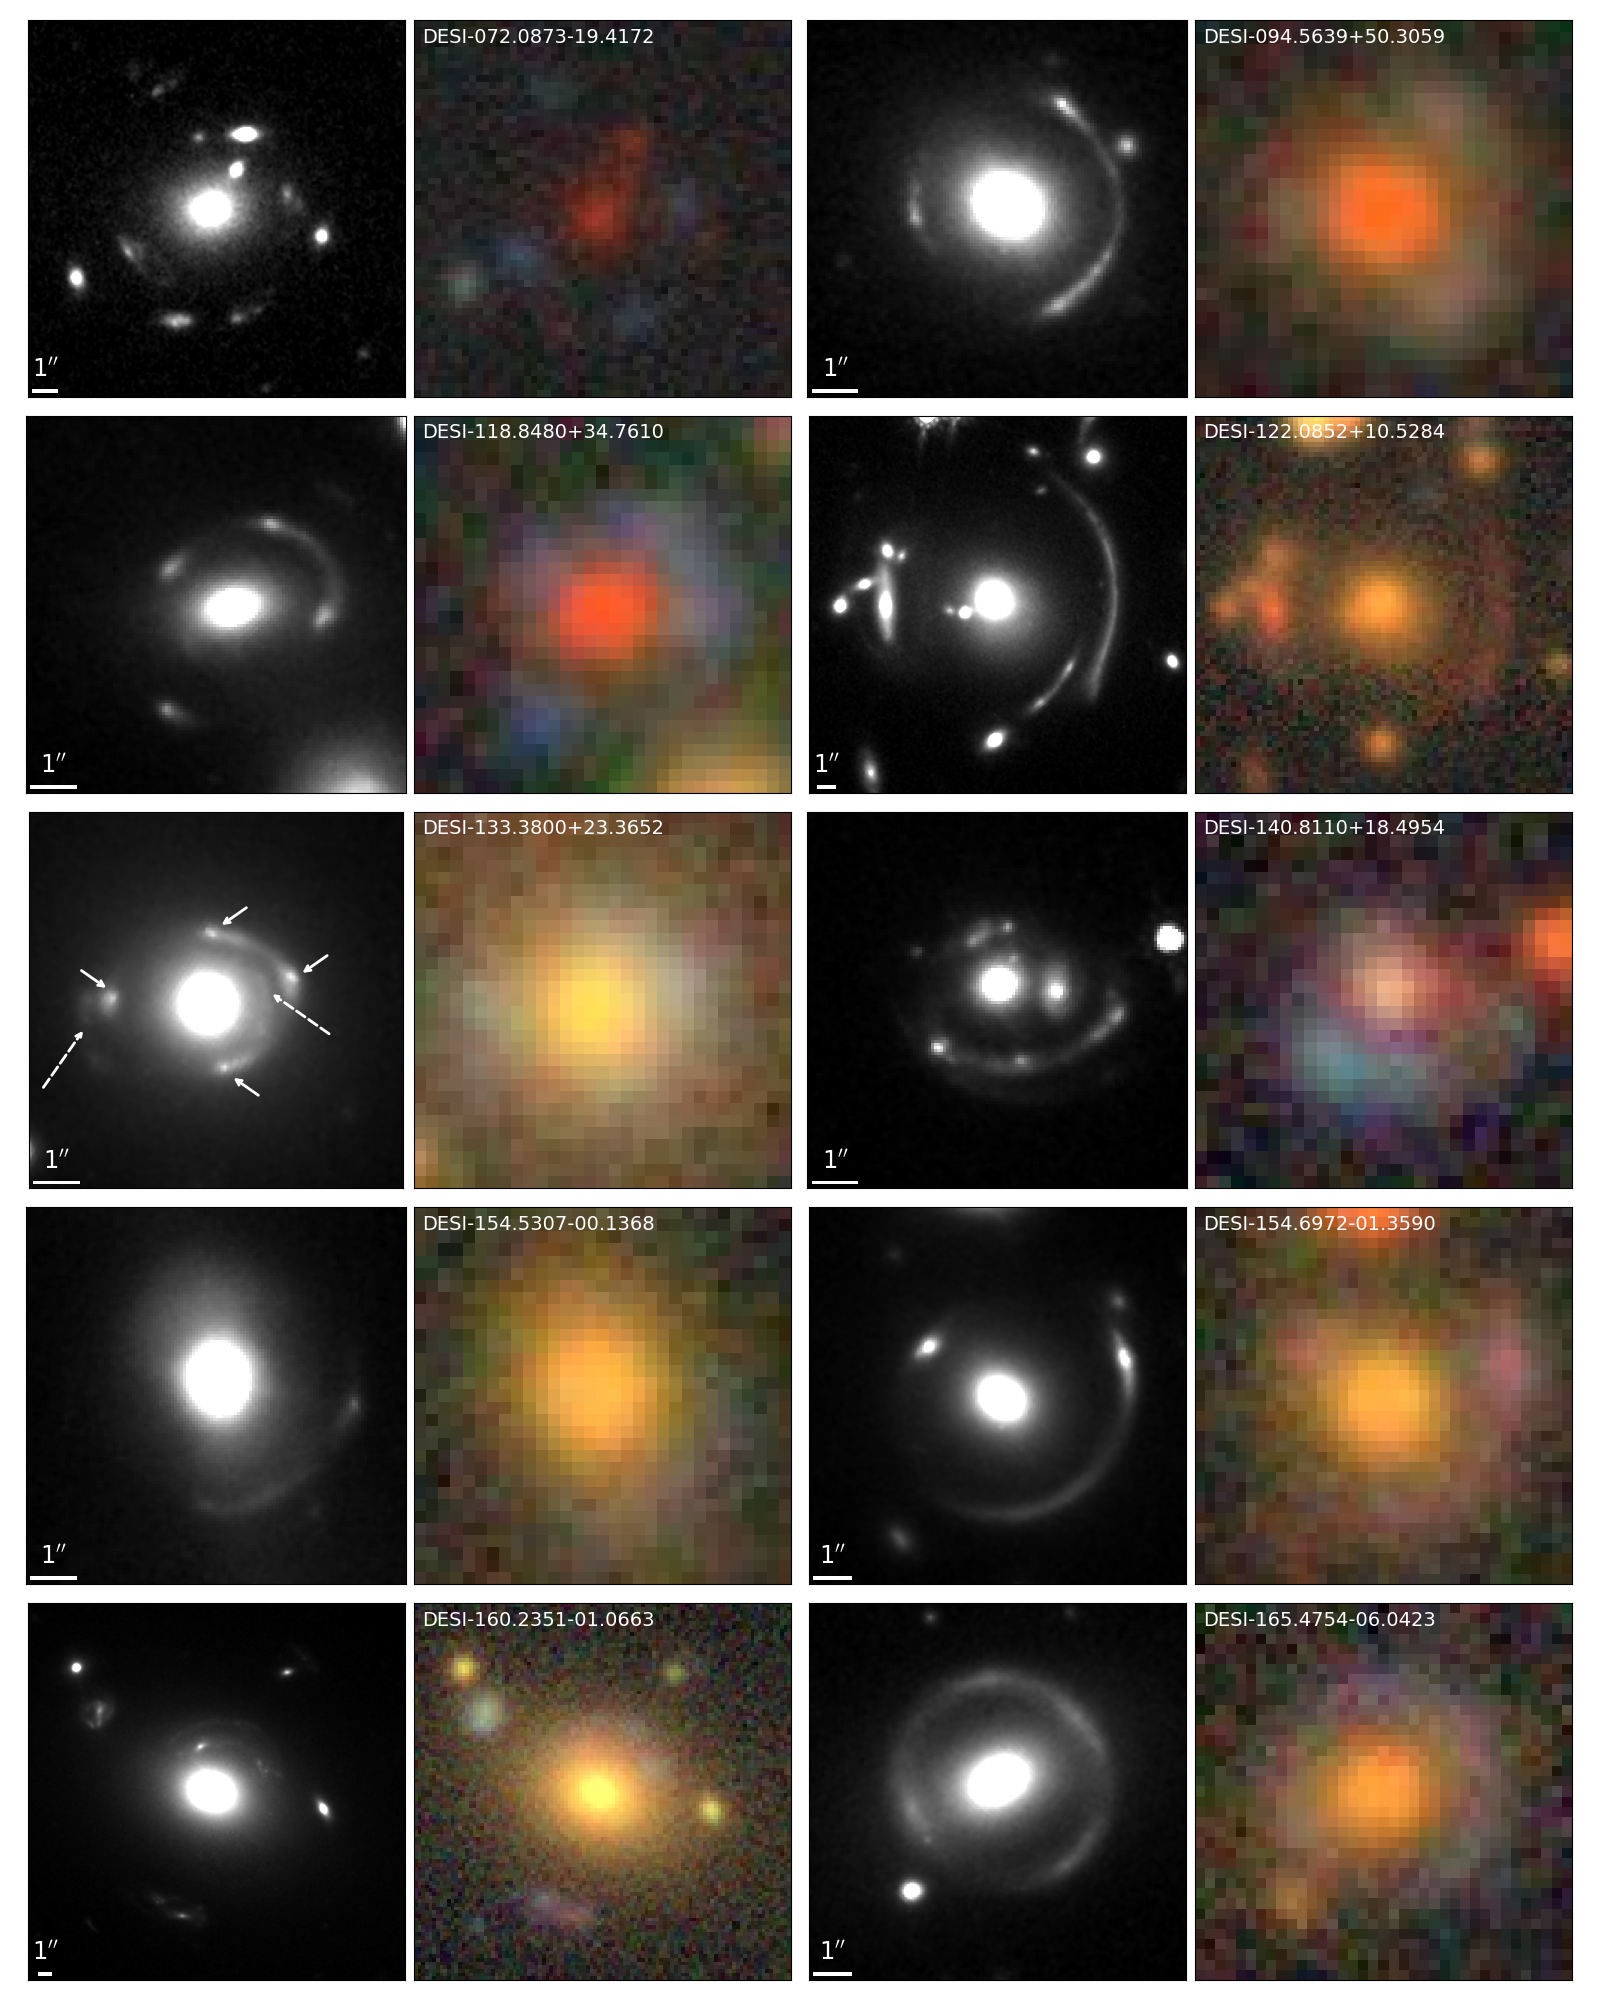
\includegraphics[keepaspectratio=true,scale=0.45]{figs/hst_panel2_arrows.png}}
% Before: hst_panel2.png
\captionof{figure}{
The next 10 (\pound9 -- \pound18) of the 51 systems in \hst GO-15867. 
For details, see the caption of Figure~\ref{fig:hstpanel-1}. 
The lens model for DESI-165.4754-06.0423 is presented in \S\,\ref{sec:lens-model}.
%Also note DESI-133.3800+23.3652, a galaxy-scale lens, likely with two lensed sources,
%which are quadruply (brighter) and doubly (fainter) lensed, respectively.
\ed{
DESI-133.3800+23.3652 is a galaxy-scale lens, likely with two sources: one quadruply lensed (solid arrows) and one doubly lensed (dashed arrows).
}
}
\label{fig:hstpanel-2}
\end{minipage}



\begin{minipage}{\linewidth}
\makebox[\linewidth]{  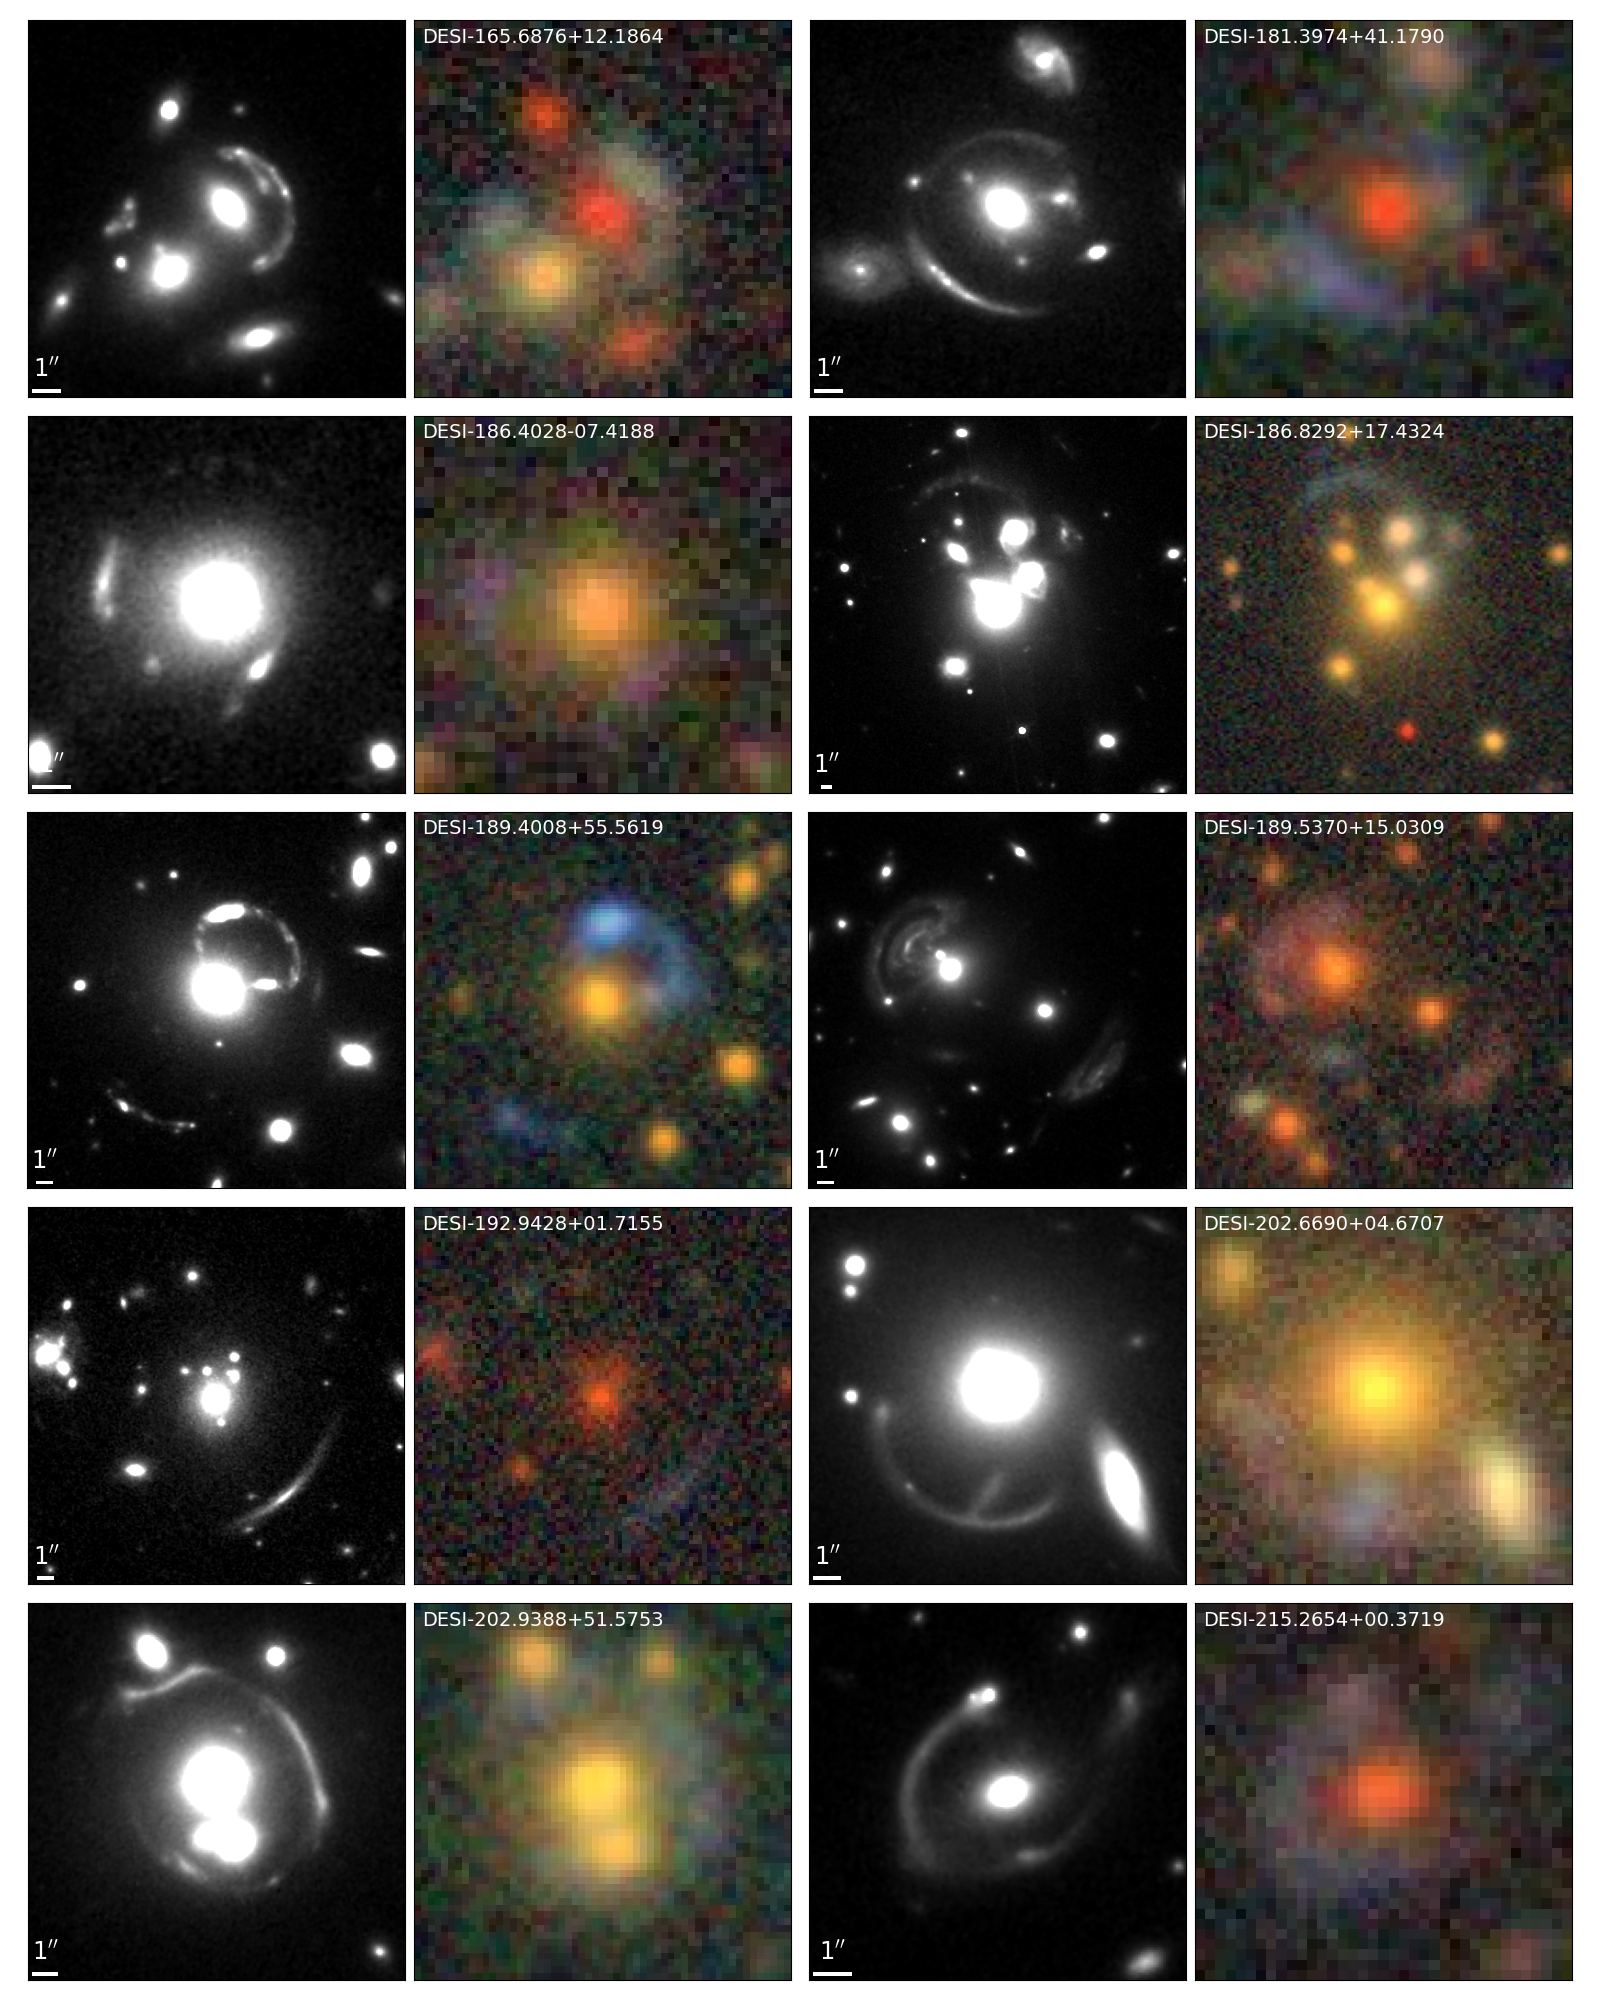
\includegraphics[keepaspectratio=true,scale=0.45]{figs/hst_panel3.png}}
\captionof{figure}{
Systems \pound19 - \pound28 of the 51 in \hst GO-15867. 
For details, see the caption of Figure~\ref{fig:hstpanel-1}.
Note that DESI 189.5370+15.0309 shows a doubly imaged background spiral galaxy with complex structure, 
resembling two half ``cinnamon buns", 
with different sizes.}
\label{fig:hstpanel-3}
\end{minipage}

\begin{minipage}{\linewidth}
\makebox[\linewidth]{  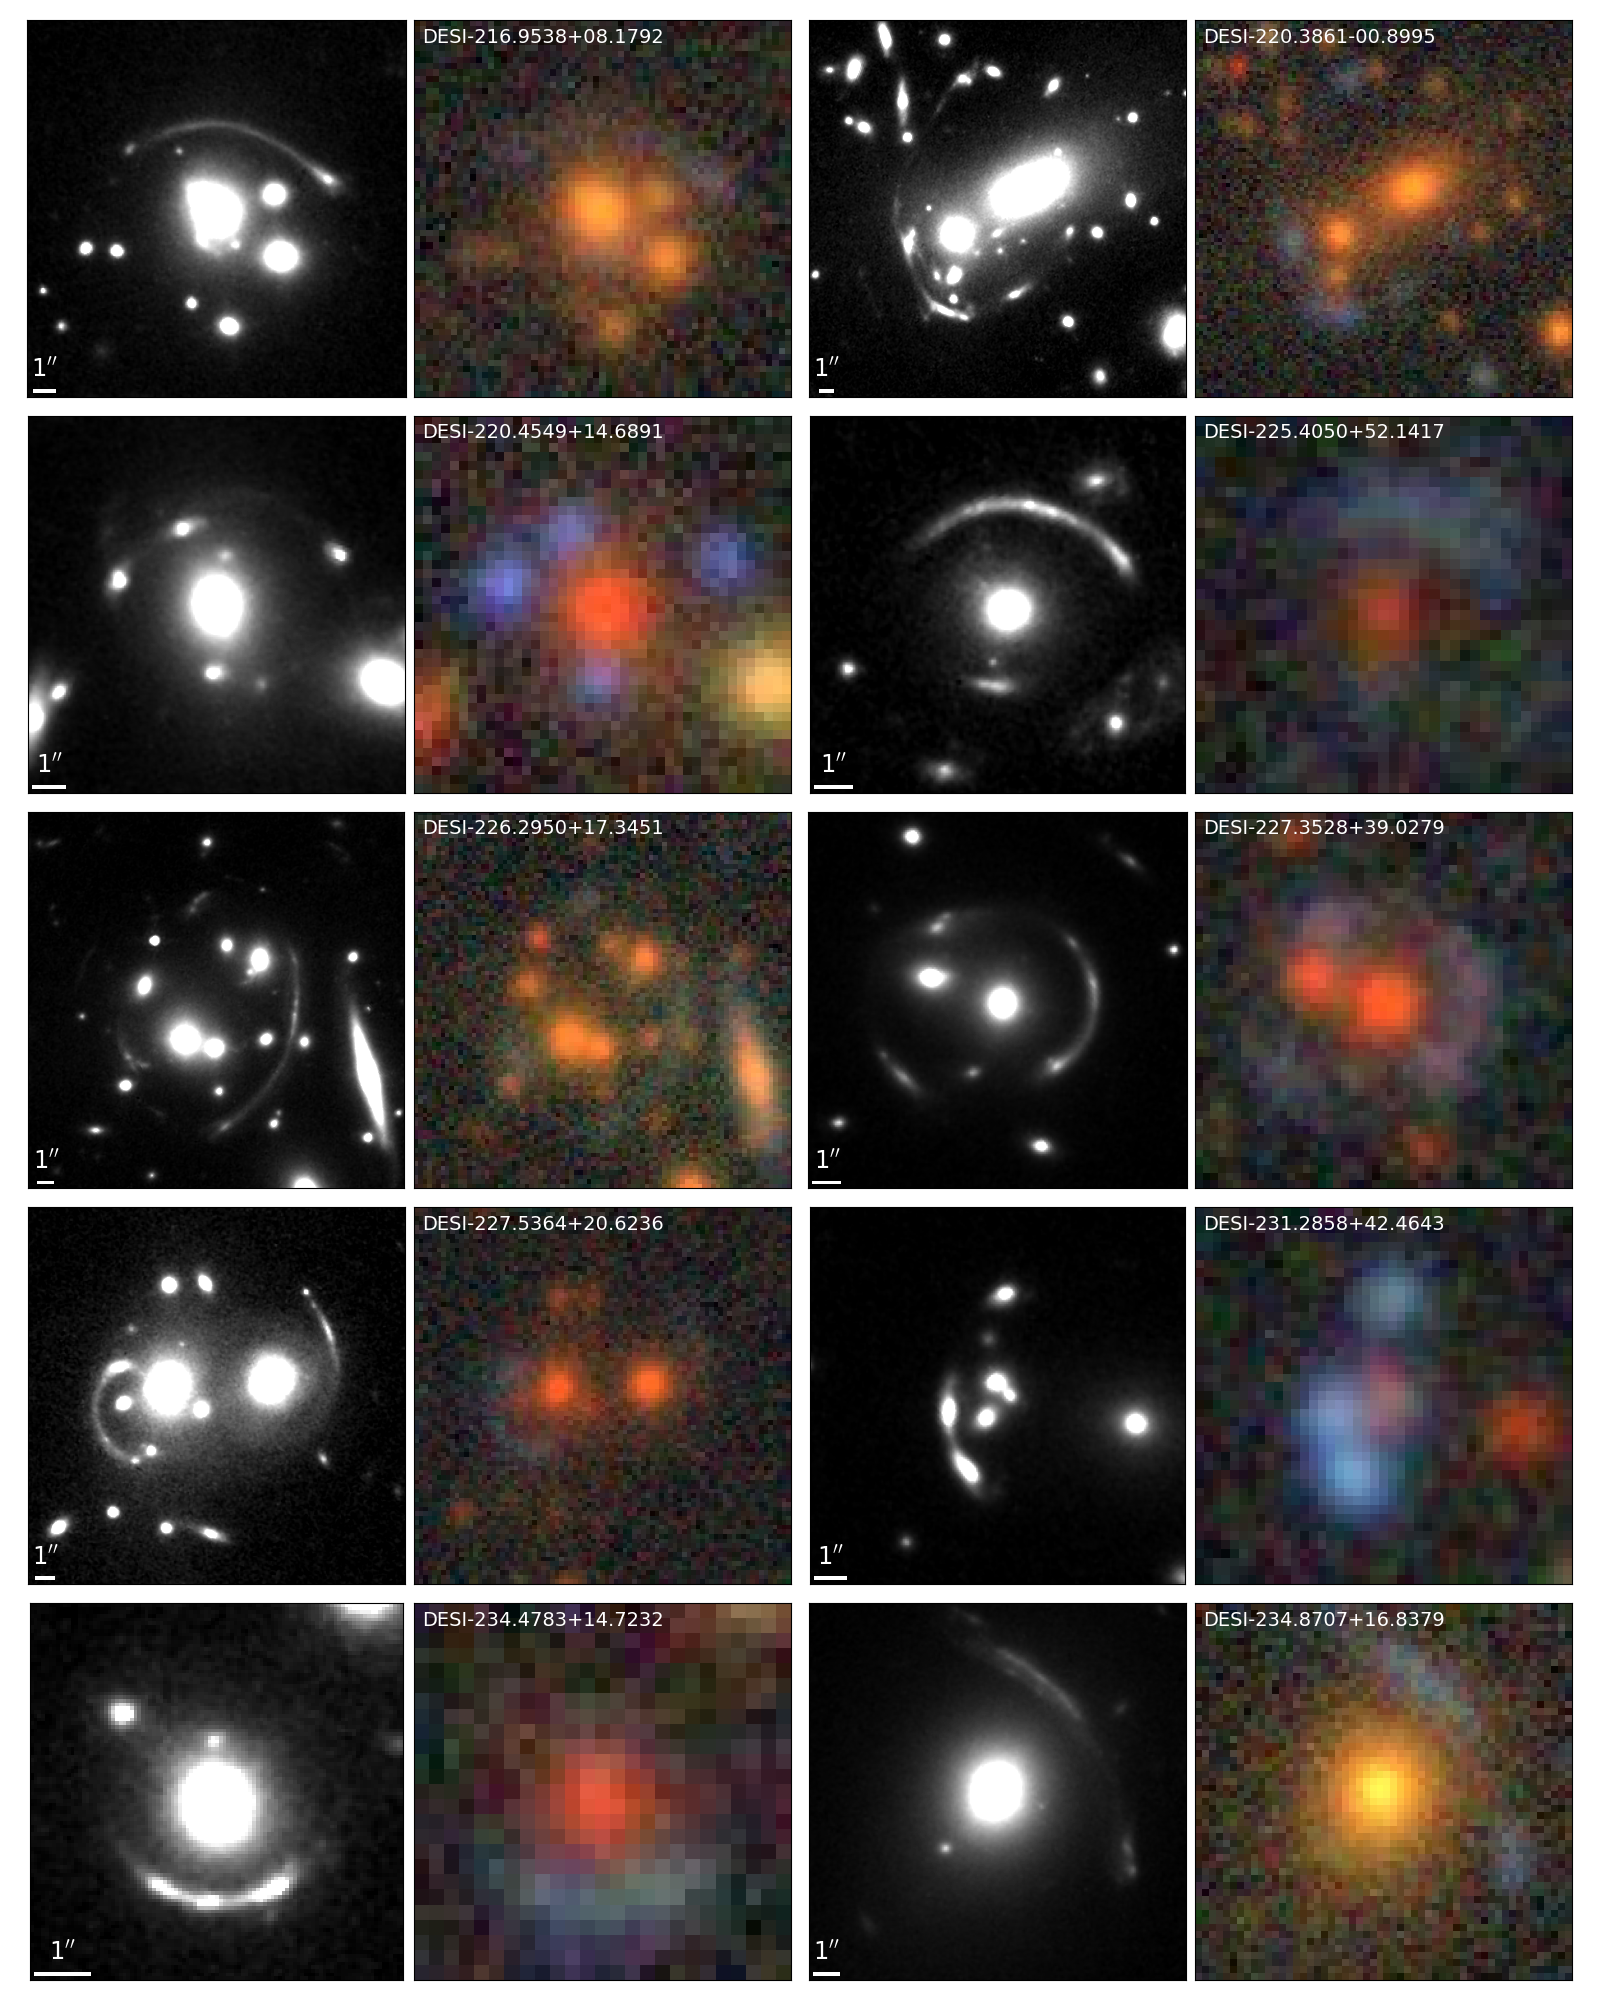
\includegraphics[keepaspectratio=true,scale=0.45]{figs/hst_panel4.png}}
\captionof{figure}{
Systems \pound29 -- \pound38 of the 51 in \hst GO-15867. For details, see the caption of Figure~\ref{fig:hstpanel-1}.}
\label{fig:hstpanel-4}
\end{minipage}

\begin{minipage}{\linewidth}
\makebox[\linewidth]{  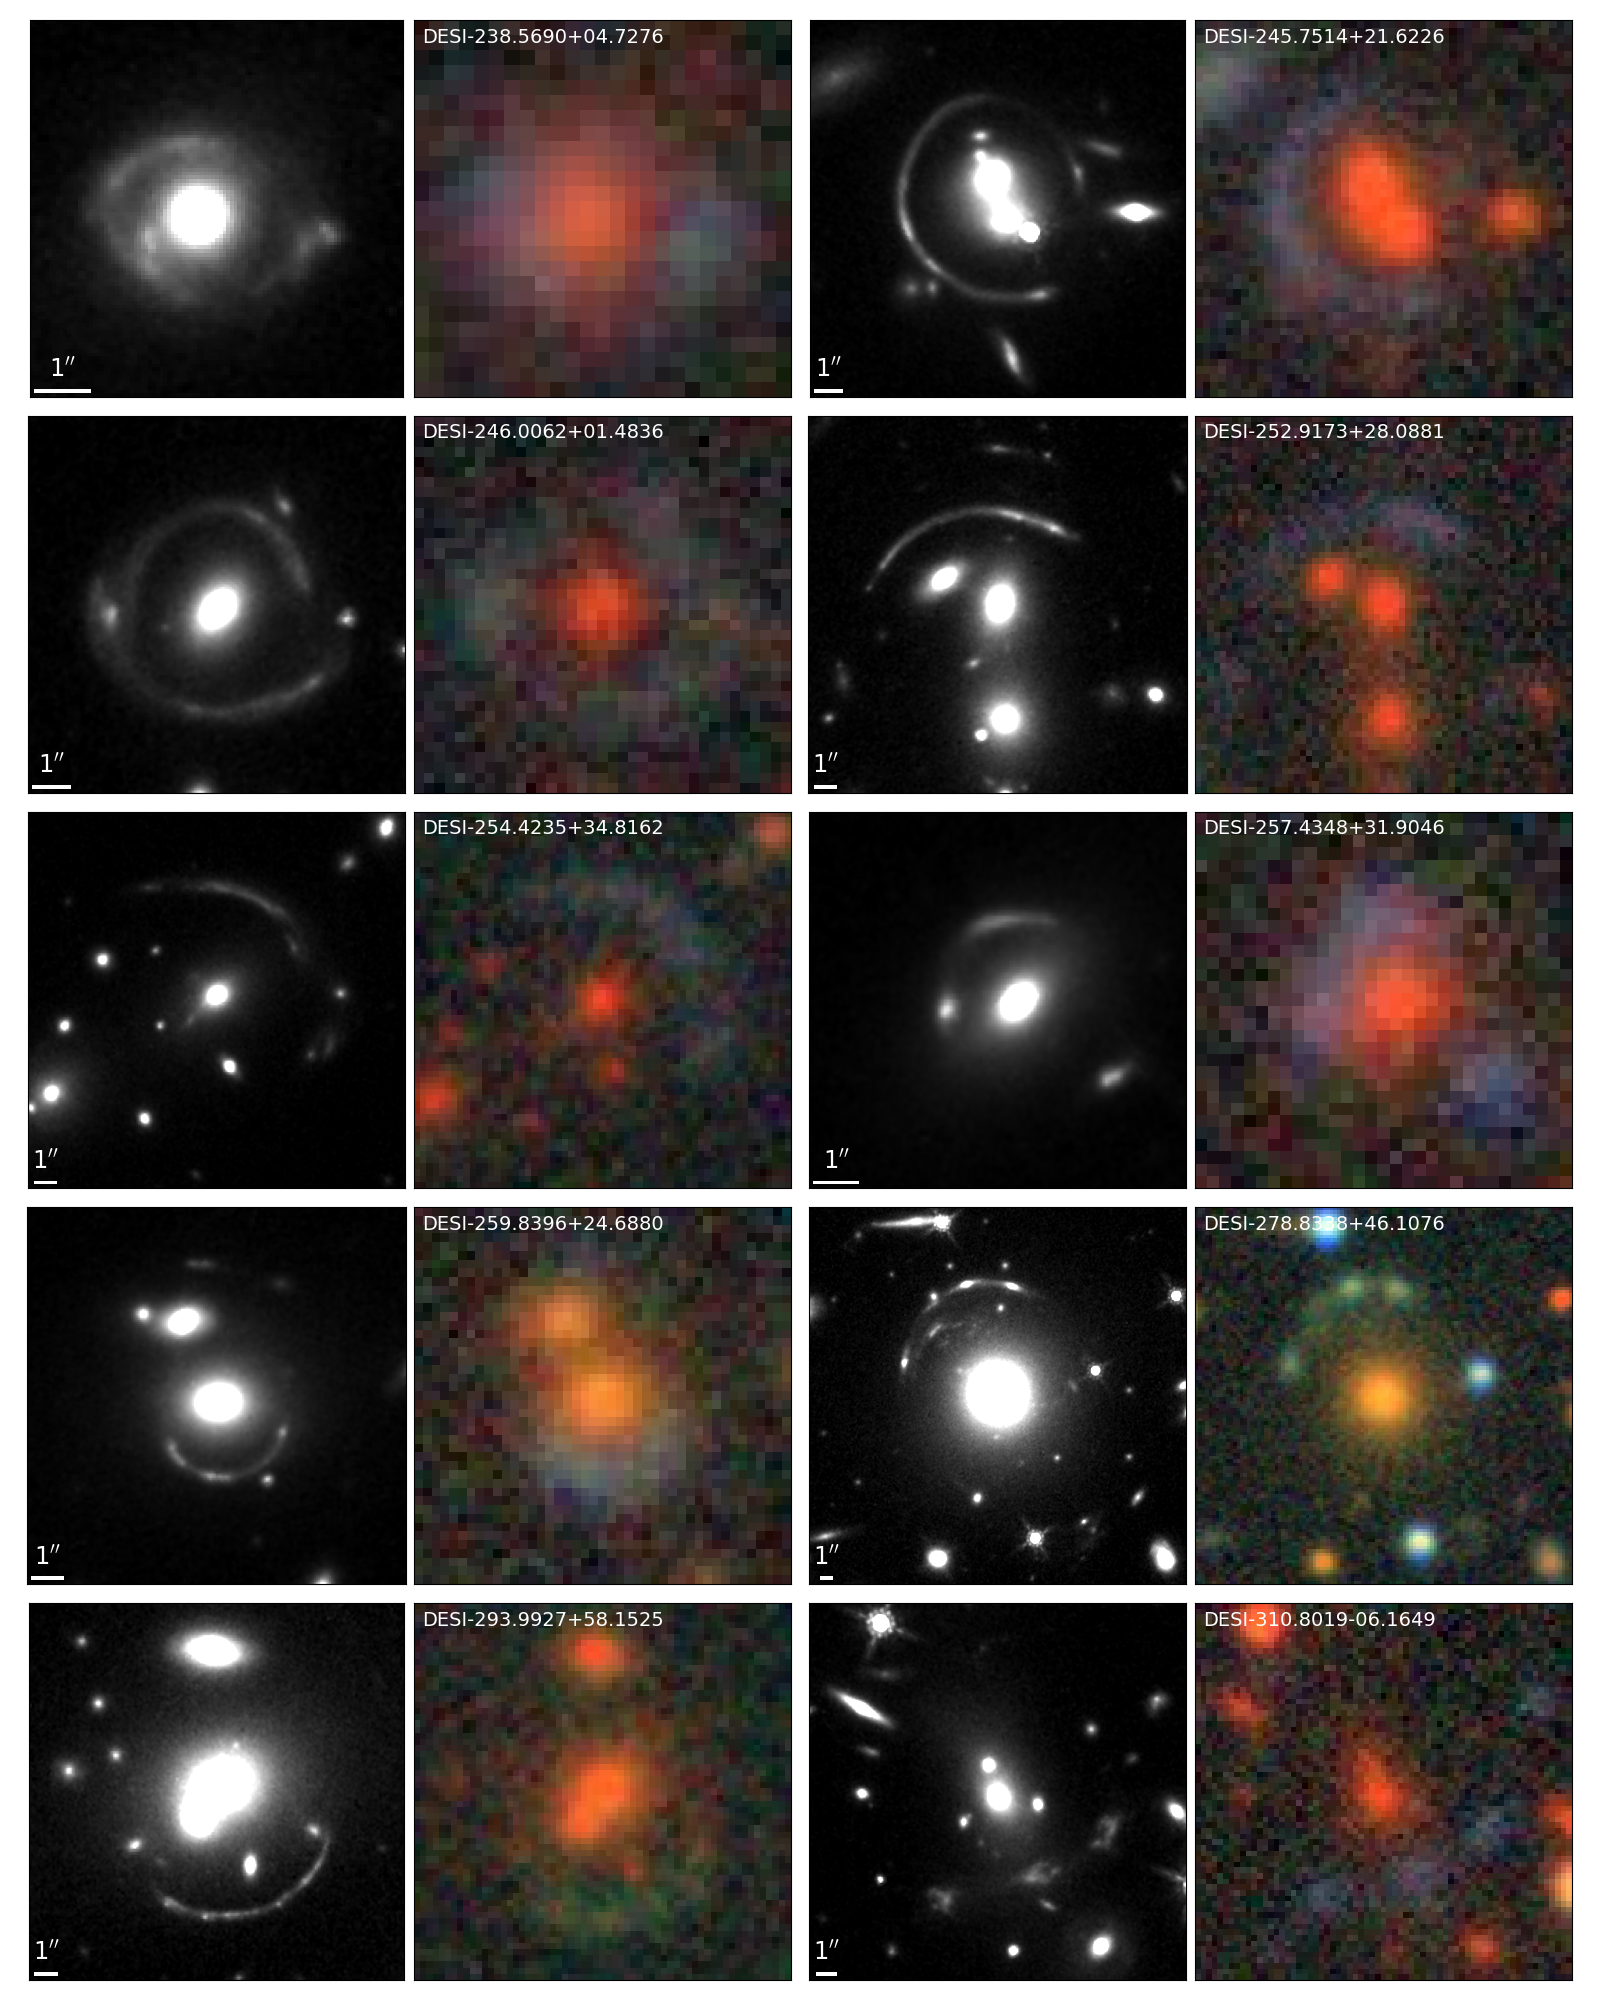
\includegraphics[keepaspectratio=true,scale=0.45]{figs/hst_panel5.png}}
\captionof{figure}{
Systems \pound39 -- \pound48 of the 51 in \hst GO-15867. 
For details, see the caption of Figure~\ref{fig:hstpanel-1}.
Note DESI-238.5690+04.7276, a galaxy-scale lens, 
likely with two lensed sources,
which are quadruply (fainter) and doubly (brighter) lensed, respectively.
%For DESI-278.8338+46.1076, \hst certainly confirmed the most prominent arc, but likely there is another arc just a little below the first arc,
%with their respective possible counterarcs near the SW corner of the cutout images (for a more detailed discussion, see text).
}
\label{fig:hstpanel-5}
\end{minipage}

\begin{minipage}{\linewidth}
\makebox[\linewidth]{  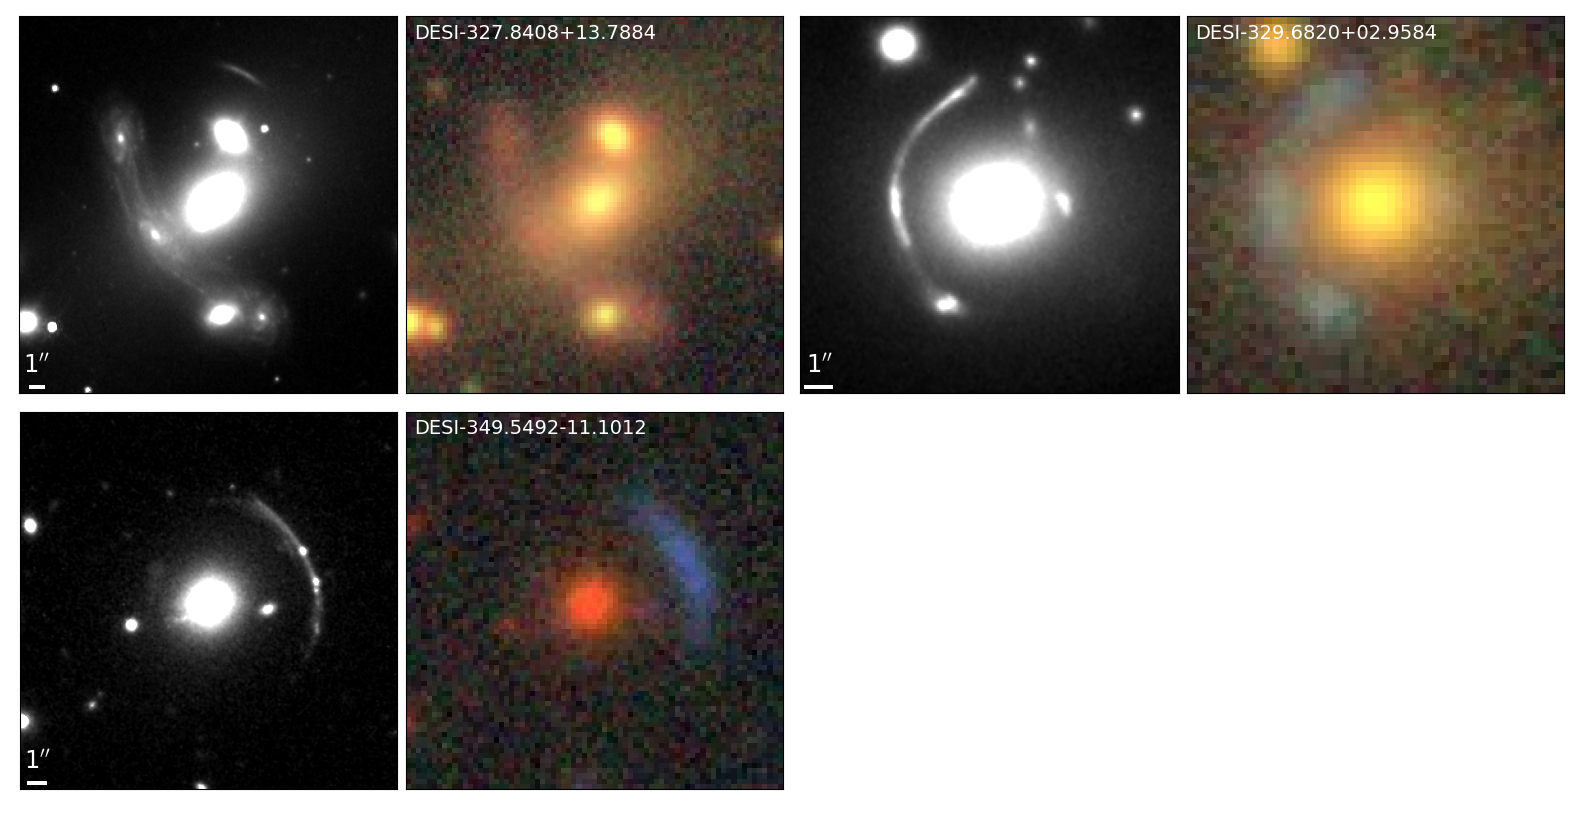
\includegraphics[keepaspectratio=true,scale=0.45]{figs/hst_panel6_revisited.png}}
\captionof{figure}{
Systems \pound49 - \pound51 of the 51 in \hst GO-15867. 
For details, see the caption of Figure~\ref{fig:hstpanel-1}.
Note that DESI-327.8408+13.7884 shows a triply lensed galaxy around a group lens \ed{(see text)}, revealing great details of the magnified background spiral galaxy.}
\label{fig:hstpanel-6}
\end{minipage}



%%%% From James
% We use \texttt{photutils} to obtain preliminary aperture photometry for the 51 systems. We first subtract the background level computed by taking the median flux of the entire field. Afterward, for each lens and arc, we visually determine and select the appropriate aperture radii from the STScI IR Encircled Energy Tables. We apply the corresponding aperture correction to obtain the final photometry.
% We present the photometry of all 51 systems in Table~\ref{tab:phot}.

\clearpage
% \startlongtable
% \begin{deluxetable*}{lccccccccc}
% \tabletypesize{\scriptsize}
% \tablecaption{\hst SNAP Targets\label{tab:phot}}
% \tablehead{
%     \colhead{Name} &
%     \colhead{Type} &
%     \colhead{F140W} &
%     \colhead{mag\_g} &
%     \colhead{mag\_r} &
%     \colhead{mag\_z} &
%     \colhead{Human} &
%     \colhead{Probability} &
%     \colhead{$z_{spec}$}&
%     \colhead{$z_{phot}$}
% }
% \startdata
% DESI-004.2564-10.1530 &	 DC &	18.79	&	21.22 &	19.52 &	18.29 & 3(0) &	0.60 &  0.00  & 0.414±0.080 \\
% DESI-002.0299+18.3723 &   DC & 17.76 & 20.63 &  19.16 &  17.84 &  0.00 &  0.97 &  0.4724 &                 \\
% \enddata
% \tablecomments{The 51 systems observed by the \hst program GO-15867.
% }
% \end{deluxetable*}

We present \hst photometry for the brightest lensed source images \ed{for the source identified in the discovery image}\footnote{\ed{As noted above, in some cases, \hst NIR observations revealed additional lensed sources. These are typically significantly fainter and their photometry is not presented here.}} for all 51 systems in Table~\ref{tab:hst-phot}, 
\ed{where we define the contour to be
at 75\% of the peak pixel value}.
To account for the luminosity contribution from the lens we employ GALFIT \citep{Peng2010a}, a parametric 2D fitting algorithm.  
We model the 
light components of the lensing galaxy using 
the S\'ersic luminosity profile \citep{sersic1963a}. Each S\'ersic component in the fitting algorithm is described by the \ed{7 parameters}: $(x,y)$ position, integrated magnitude $m$, effective radius $r_e$, concentration index $n$, axis ratio $q$, and position angle $\theta$.
\par Prior to the fitting procedure, a PSF was generated for each image by stacking star cutouts from the field and iteratively refining a proposed PSF model based on the stack. This process was carried out using \texttt{PSFr} 
% (Birrer et al. in prep) 
% utilizing features of 
in the \texttt{Lenstronomy} package \citep{birrer2021a}. Following successful extraction of PSFs, each galaxy was initially fit \ed{using} a single S\'ersic component, with additional components added when necessary to adequately subtract the lens light from the image. Goodness of fit was determined using the $\chi^2$ metric as well as visual inspection of the image residuals. In cases where model parameters deviated from physically acceptable values, such as extreme $r_e$, constraints were imposed. For systems where the lensing field was densely populated, the light profiles of all galaxies in the image region were also modeled and subtracted to reduce contamination of source light. Moreover, in certain outlier cases where 
% images from two sources 
two source images appeared in close proximity to each other, the source light for such systems was also modeled in order to properly isolate each source image. Source light distribution was modeled using \ser profiles along with an additional bending mode where necessary.


\startlongtable
\begin{deluxetable*}{lcccc}
\tabletypesize{\scriptsize}
\tablecaption{Isophotal magnitudes for the brightest source image
% for all 51 systems. 
% For systems with two entries, each magnitude corresponds to a different image family.
\label{tab:hst-phot}}
\tablehead{
    \colhead{Target Name} &
    \colhead{\ed{RA (deg)}} &
    \colhead{\ed{Dec (deg)}} &
    \colhead{F140W Isophotal Magnitude \ed{(AB mag)}} &
    \colhead{Contour Area \ed{(arcsec$^2$)}} 
}
\startdata
DESI-004.2564-10.1530 & 4.2560 & $-$10.1549 & 23.51 $\pm$ 0.02 & 0.0380 \\
DESI-006.3643+10.1853 & 6.3646 & 10.1820 & 23.79 $\pm$ 0.02 & 0.0338 \\
DESI-023.0157-16.0040 & 23.0152 & $-$16.0041 & 25.04 $\pm$ 0.04 & 0.0634 \\
DESI-023.6765+04.5639 & 23.6753 & 4.5635 & 25.68 $\pm$ 0.05 & 0.0338 \\
DESI-024.1631+00.1384 & 24.1628 & 0.1376 & 24.89 $\pm$ 0.04 & 0.0380 \\
DESI-025.4848+30.7585 & 25.4846 & 30.7587 & 26.43 $\pm$ 0.07 & 0.0423 \\
DESI-030.4360-27.6618 & 30.4365 & $-$27.6617 & 25.43 $\pm$ 0.05 & 0.0211 \\
DESI-033.8095-29.1570 & 33.8094 & $-$29.1571 & 24.16 $\pm$ 0.03 & 0.0169 \\
DESI-072.0873-19.4172 & 72.0883 & $-$19.4177 & 26.20 $\pm$ 0.06 & 0.0296 \\
DESI-094.5639+50.3059 & 94.5634 & 50.3065 & 24.88 $\pm$ 0.04 & 0.0211 \\
DESI-118.8480+34.7610 & 118.8477 & 34.7615 & 24.64 $\pm$ 0.03 & 0.0338 \\
DESI-122.0852+10.5284 & 122.0836 & 10.5279 & 22.43 $\pm$ 0.01 & 0.5197 \\
DESI-133.3800+23.3652 & 133.3795 & 23.3653 & 23.98 $\pm$ 0.02 & 0.0296 \\
DESI-140.8110+18.4954 & 140.8114 & 18.4951 & 24.35 $\pm$ 0.03 & 0.0423 \\
DESI-154.5307-00.1368 & 154.5299 & $-$0.1369 & 25.42 $\pm$ 0.05 & 0.0296 \\
DESI-154.6972-01.3590 & 154.6977 & $-$1.3587 & 23.24 $\pm$ 0.02 & 0.0296 \\
DESI-160.2351-01.0663 & 160.2353 & $-$1.0654 & 23.55 $\pm$ 0.02 & 0.0423 \\
DESI-165.4754-06.0423 & 165.4760 & $-$6.0425 & 23.87 $\pm$ 0.02 & 0.1394 \\
DESI-165.6876+12.1864 & 165.6870 & 12.1865 & 25.02 $\pm$ 0.04 & 0.0211 \\
DESI-181.3974+41.1790 & 181.3981 & 41.1783 & 24.47 $\pm$ 0.03 & 0.0465 \\
DESI-186.4028-07.4188 & 186.4026 & $-$7.4193 & 24.92 $\pm$ 0.04 & 0.0296 \\
DESI-186.8292+17.4324 & 186.8287 & 17.4343 & 24.13 $\pm$ 0.02 & 0.2113 \\
%\ed{DESI-189.4008+55.5619a} & 189.4004 & 55.5633 & 22.64 $\pm$ 0.01 & 0.0718 \\
DESI-189.4008+55.5619 & 189.4036 & 55.5601 & 24.26 $\pm$ 0.03 & 0.0380 \\
DESI-189.5370+15.0309 & 189.5388 & 15.0313 & 23.81 $\pm$ 0.02 & 0.0676 \\
DESI-192.9428+01.7155 & 192.9417 & 1.7138 & 23.59 $\pm$ 0.02 & 0.1648 \\
DESI-202.6690+04.6707 & 202.6700 & 4.6698 & 23.74 $\pm$ 0.02 & 0.1310 \\
DESI-202.9388+51.5753 & 202.9371 & 51.5752 & 23.32 $\pm$ 0.02 & 0.1817 \\
DESI-215.2654+00.3719 & 215.2652 & 0.3715 & 24.39 $\pm$ 0.03 & 0.0845 \\
DESI-216.9538+08.1792 & 216.9525 & 8.1795 & 24.21 $\pm$ 0.03 & 0.0507 \\
DESI-220.3861-00.8995 & 220.3884 & $-$0.9006 & 23.94 $\pm$ 0.02 & 0.0507 \\
% \ed{DESI-220.3861-00.8995b} & 220.3878 & $-$0.9018 & 23.93 $\pm$ 0.02 & 0.0465 \\
% \ed{DESI-220.3861-00.8995c} & 220.3874 & $-$0.8974 & 24.56 $\pm$ 0.03 & 0.0296 \\
DESI-220.4549+14.6891 & 220.4557 & 14.6893 & 23.74 $\pm$ 0.02 & 0.0338 \\
DESI-225.4050+52.1417 & 225.4047 & 52.1424 & 24.97 $\pm$ 0.04 & 0.0380 \\
DESI-226.2950+17.3451 & 226.2932 & 17.3455 & 24.68 $\pm$ 0.03 & 0.0549 \\
DESI-227.3528+39.0279 & 227.3521 & 39.0273 & 23.91 $\pm$ 0.02 & 0.0507 \\
DESI-227.5364+20.6236 & 227.5339 & 20.6244 & 23.74 $\pm$ 0.02 & 0.1099 \\
DESI-231.2858+42.4643 & 231.2877 & 42.4639 & 23.08 $\pm$ 0.02 & 0.0465 \\
DESI-234.4783+14.7232 & 234.4780 & 14.7227 & 25.12 $\pm$ 0.04 & 0.0254 \\
DESI-234.8707+16.8379 & 234.8703 & 16.8391 & 24.47 $\pm$ 0.03 & 0.0803 \\
DESI-238.5690+04.7276 & 238.5695 & 4.7277 & 24.24 $\pm$ 0.03 & 0.1352 \\
DESI-245.7514+21.6226 & 245.7524 & 21.6224 & 23.71 $\pm$ 0.02 & 0.0887 \\
%\ed{DESI-246.0062+01.4836a} & 246.0070 & 1.4836 & 24.28 $\pm$ 0.03 & 0.0718 \\
DESI-246.0062+01.4836 & 246.0060 & 1.4843 & 24.97 $\pm$ 0.04 & 0.0803 \\
%\ed{DESI-246.0062+01.4836c} & 246.0056 & 1.4831 & 25.54 $\pm$ 0.05 & 0.0338 \\
DESI-252.9173+28.0881 & 252.9166 & 28.0890 & 24.45 $\pm$ 0.03 & 0.0634 \\
DESI-254.4235+34.8162 & 254.4234 & 34.8174 & 24.00 $\pm$ 0.02 & 0.1732 \\
DESI-257.4348+31.9046 & 257.4352 & 31.9046 & 24.13 $\pm$ 0.02 & 0.0380 \\
DESI-259.8396+24.6880 & 259.8397 & 24.6873 & 24.94 $\pm$ 0.04 & 0.0338 \\
%DESI-259.8396+24.6880$^{b}$ & 259.8398 & 24.6891 & 25.97 $\pm$ 0.06 & 0.0296 \\
DESI-278.8338+46.1076 & 278.8348 & 46.1099 & 23.52 $\pm$ 0.02 & 0.0423 \\
DESI-293.9927+58.1525 & 293.9930 & 58.1510 & 26.15 $\pm$ 0.06 & 0.0211 \\
DESI-310.8019-06.1649 & 310.8015 & $-$6.1660 & 23.86 $\pm$ 0.02 & 0.1648 \\
DESI-327.8408+13.7884 & 327.8425 & 13.7896 & 23.67 $\pm$ 0.02 & 0.0465 \\
%\ed{DESI-329.6820+02.9584a} & 329.6825 & 2.9575 & 23.92 $\pm$ 0.02 & 0.0380 \\
%\ed{DESI-329.6820+02.9584b} & 329.6830 & 2.9584 & 23.94 $\pm$ 0.02 & 0.0465 \\
% We chose c, b/c Tran22 targeted b+c
DESI-329.6820+02.9584 & 329.6824 & 2.9595 & 23.91 $\pm$ 0.02 & 0.0592 \\
DESI-349.5492-11.1012 & 349.5478 & $-$11.1005 & 25.33 $\pm$ 0.04 & 0.0085 \\
\enddata
\end{deluxetable*}


% \input{photometry}